\subsection*{Task 5.3}

The Lagrange basis polynomials for l = 3 are calculated as:

\begin{align*}
	L_i(x) = \frac{(x-x_0)(x-x_1)(x-x_2)(x-x_3)}{(x_i-x_0)(x_i-x_1)(x_i-x_2)(x_i-x_3)}
\end{align*}

With our data points

\begin{align*}
x_0 &= 0, y_0 = 1\\
x_1 &= 1, y_1 = 3\\
x_2 &= 3, y_2 = -2\\
x_3 &= 5, y_3 = 4\
\end{align*}

we receive:

\begin{align*}
L_0(x) &= \frac{(x-1)(x-3)(x-5)}{(0-1)(0-3)(0-5)}
 = \frac{x^3-9x^2+23x-15}{-15}\\
L_1(x) &= \frac{(x-0)(x-3)(x-5)}{(1-0)(1-3)(1-5)}
 = \frac{x^3-8x^2+15x}{8}\\
L_2(x) &= \frac{(x-0)(x-1)(x-5)}{(3-0)(3-1)(3-5)}
 = \frac{x^3-6x^2+5x}{-12}\\
L_3(x) &= \frac{(x-0)(x-1)(x-3)}{(5-0)(5-1)(5-3)}
 = \frac{x^3-4x^2+3x}{40}\\
\end{align*}

The Lagrange polynomial $p_3(x)$ is calculated as:

\begin{align*}
p_3(x) &= \sum_{i=0}^{3}y_iL_i(x) \\
&= \frac{x^3-9x^2+23x-15}{-15}+ 3\cdot \frac{x^3-8x^2+15x}{8} -2\cdot \frac{x^3-6x^2+5x}{-12}+ 4\cdot \frac{x^3-4x^2+3x}{40}\\
&= \frac{23x^3}{40}-\frac{19x^2}{5}+\frac{209x}{40}+1
\end{align*}

\begin{figure}[!h]
	\centering
	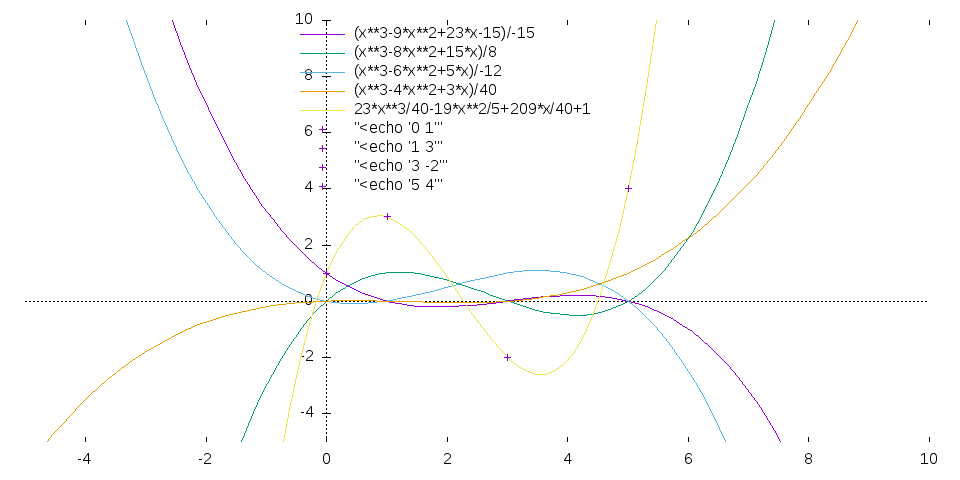
\includegraphics[width= 1\textwidth ]{task52.png}
	\caption{Langrange basis polynomials and polynomial $p_3$.}
\end{figure}